\documentclass[nobib]{MSword}
% Class options:
%-------------------------------
% nobib         - skip bibliography code/ don't include bib
% math          - include math packages and useful math commands
% hidelinks     - hide hyperref colored link boxes
% wordlinks     - link color scheme similar to word


% Preamble code:
%%%%%%%%%%%%%%%%%%%%%%%%%%%%%%%%%%%%%%%%
\usepackage[english]{babel}
\usepackage{csquotes}
\usepackage{lipsum}
\usepackage{geometry}
\usepackage{amsmath}
 \usepackage{graphicx}
 \usepackage{titling}

% % Uncomment using "Ctrl + /" (/ on numpad):
% % Customizing headers and footers:
% \fancypagestyle{custom}{%
%     \fancyhf{}% clears the footer and header
%     % Header:
%     \fancyhead[L]{}
%     \fancyhead[C]{}
%     \fancyhead[R]{}
%     % Footer:
%     \fancyfoot[L]{}
%     \fancyfoot[C]{}
%     \fancyfoot[R]{}
%         % Tips:
%         % ----
%         % L: left, C: center, R: right
%         % O: odd pages, E: even pages
%         % ----
%         % Example: \fancyghead[LO,RE]{Text}
%         % will produce "Text" left in the header
%         % on odd pages and right in the header on even pages.
%     % Rules/ lines:
%     \renewcommand{\headrulewidth}{0.4pt}
%     \renewcommand{\footrulewidth}{2pt}
% }
% % Changing the pagestyle:
% \pagestyle{custom}

%%%%%%%%%%%%%%%%%%%%%%%%%%%%%%%%%%%%%%%%

% Preamble information:
%%%%%%%%%%%%%%%%%%%%%%%%%%%%%%%%%%%%%%%%

\title{ENPM673 - Project 1 Report}
\author{Sandeep Thalapanane}
\date{UID - 119402535}

%%%%%%%%%%%%%%%%%%%%%%%%%%%%%%%%%%%%%%%%

% The document:
%%%%%%%%%%%%%%%%%%%%%%%%%%%%%%%%%%%%%%%%
\begin{document}

\maketitle
% \begin{center}
%     Words: \quickwordcount{main}\\ % Word count 
%     Pages: \pageref{LastPage} % Page count
% \end{center}

% Text files from txt folder:
\section{Ball Tracking}
   In this problem, a red ball is thrown against a wall, and using the OpenCV library we track the ball and plot the pixel coordinates of the red ball center, and also find a best-fit curve using least squares.\\
   Steps in the Execution:
   \begin{enumerate}
       \item The video is read using a cv.VideoCapture and in the next step an infinite while loop is used to read the video frame by frame using read().
       \item The color channel is changed to HSV from BGR using cv.cvtColor.
       \item To filter the red channel cv.inRange is used by specifying the upper and lower threshold limits.
       \item The pixel coordinates are extracted after filtering the red channel and the mean of x coordinates and y coordinates are found to locate the center of the ball.
       \item After finding the pixel coordinates in each frame of the video, the least squares method is used to find the best-fit curve for the coordinates.
   \end{enumerate} 

\begin{figure}[h]
    \centering
    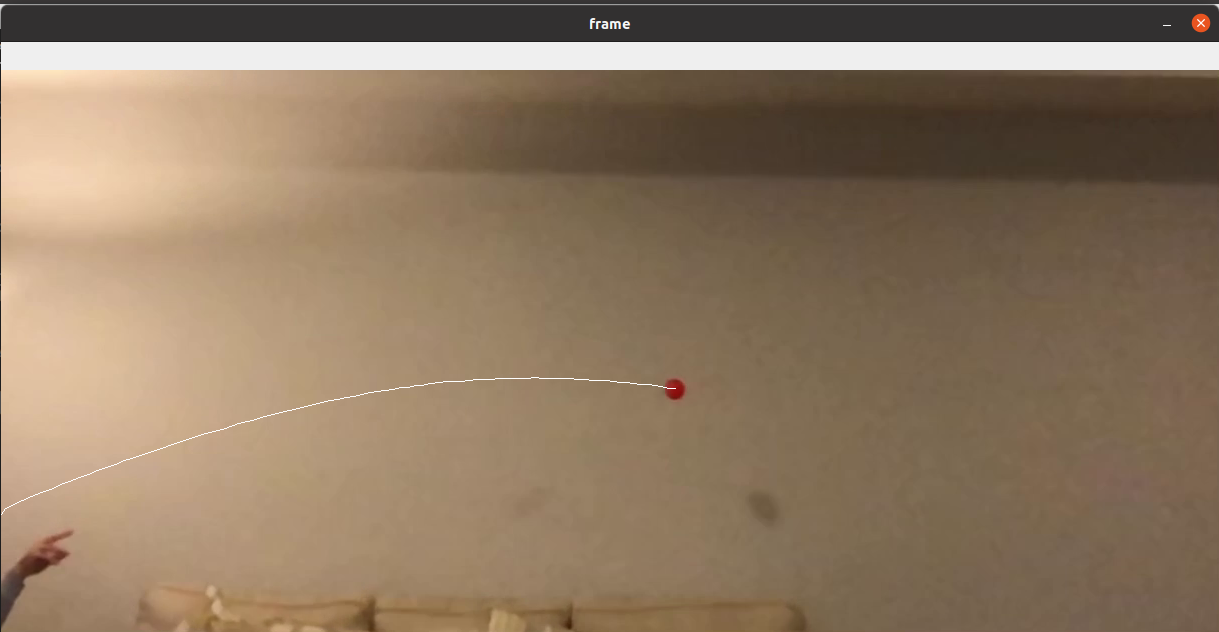
\includegraphics[width=0.75\textwidth]{txt/Proj1_balltrack.png}
    \caption{Ball tracking}
    \label{fig:my_label}
\end{figure}
\subsection{Least squares}
  In the least squares method, we find the best-fit curve by reducing the mean square error. The general equation for a parabola is $y = ax^2 + bx + c$. 
  The error is calculated in the vertical direction only and the equation is $E = \sum_{i=1}^{N} (y_i - ax{_i}{^2} - bx_i - c)$.\\
The error equation in the matrix form is $E = \| Y - XB \|^{2}$, where  \vspace{8mm} \\
  $Y =
  \begin{pmatrix}
    y_1 \\
    y_2 \\
     \vdots \\
    y_n
  \end{pmatrix}$ 
$ X =
  \begin{pmatrix}
    x{_1}{^2} & x{_1} & 1 \\
    x{_2}{^2} & x{_2} & 1 \\
     \vdots & \vdots & \vdots\\ 
    x{_n}{^2} & x{_n} & 1
  \end{pmatrix}$ 
$ B =
  \begin{pmatrix}
    a \\
    b \\
    c
  \end{pmatrix}$   \vspace{8mm} \\
After differentiating the error equation w.r.t B, equating it to zero, and after solving we get \\
$B = (X^T X)^{-1} (X^T Y)$. \\
Coefficients a, b, and c of the parabola equation are calculated using the above equation, and the x, and y pixel coordinates of the center of the ball and the curve is plotted using those coefficients.\\
The equation of the curve is $y =  0.000591548452322787 x^2  - 0.5997959453537174 x + 456.82090742179395$ \\
After finding the equation of the curve, the x coordinate of the ball's landing spot is fetched by giving the sum of the first y coordinate and 300 as input and then solving the quadratic equation. There are 2 possible points from the curve equation, since the pixel coordinate cannot be negative, it is neglected and the x coordinate of the ball's landing spot is the positive value which is 1369.
\begin{figure}[!h]
    \centering
    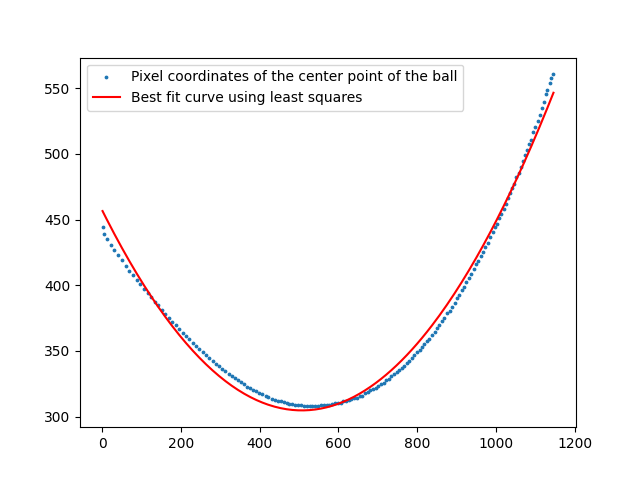
\includegraphics[width=0.75\textwidth]{txt/Proj1_1.png}
    \caption{Pixel coordinates and best-fit curve to predict trajectory}
    \label{fig:my_label} 
\end{figure} 

\section{Covariance matrix, LS, TLS and RANSAC}
\subsection{Covariance matrix and Surface normal}
  Covariance is a measure of the joint variability of two random variables. Covariance between two same variables is called variance. The covariance of two variables (x,y) is found by using the below equation - \\
$cov(x,y) = \frac{1}{n} (\sum (x - \Bar{x})(y - \Bar{y}))$, where $\Bar{x} \text{ and } \Bar{y}$ are the mean values of x and y respectively\\
 The covariance matrix for 3D data is given by:
 $
 \begin{pmatrix}
     cov(x, x) & cov(x, y) & cov(x, z) \\
     cov(y, x) & cov(y, y) & cov(y, z) \\
     cov(z, x) & cov(z, y) & cov(z, z)
 \end{pmatrix}
 $ \\ 
The covariance matrix for the PS1 data set is :
$
\begin{pmatrix}
    33.7500586 &   -0.82513692 & -11.39434956 \\
    -0.82513692 &  35.19218154 & -23.23572298 \\
    -11.39434956 & -23.23572298  & 20.62765365 
\end{pmatrix} $  \vspace{5mm} \\
The magnitude and the direction of the surface normal were calculated using the covariance matrix eigenvalues and eigen vector. The direction of the surface normal is given by the eigen vector corresponding to the smallest eigenvalue of the covariance matrix of the data set. The direction of the surface normal is (0.28616428, 0.53971234, 0.79172003) and the magnitude is 1.

\subsection{Standard Least squares for 3D point cloud}
  As mentioned above in the least squares method, we find the best-fit surface plane by reducing the mean square error. The general equation for a surface is $z = ax + by + c$. 
  The error is calculated as $E = \sum_{i=1}^{N} (z_i - ax{_i} - by_i - c){^2}$.\\
The error equation in the matrix form is $E = \| Z - XB \|^{2}$, where \vspace{3mm}  \\
  $Z =
  \begin{pmatrix}
    z_1 \\
    z_2 \\
    \vdots \\
    z_n
  \end{pmatrix}$ 
$ X =
  \begin{pmatrix}
    x{_1} & y{_1} & 1 \\
    x{_2} & y{_2} & 1 \\
    \vdots & \vdots & \vdots \\
    z{_n}{^2} & y{_n} & 1
  \end{pmatrix}$ 
$ B =
  \begin{pmatrix}
    a \\
    b \\
    c
  \end{pmatrix}$ \vspace{5mm} \\
The error is found only in the z-axis direction in this method.
After differentiating the error equation w.r.t B, equating it to zero, and after solving we get, \\
$B = (X^T X)^{-1} (X^T Y)$ \\
Using the above equation and the x, y, and z points of the data set, coefficients a, b, and c of the surface equation are found and the surface plane is plotted.
\subsection{Total Least squares for 3D point cloud}
 In the standard least squares method, the error is only found in one direction and if the points lie in the same direction as the error-calculated direction, then the least squares might not produce good results. Whereas in the total least squares method, the error is found orthogonally to the plane, and the error is minimized to find the best-fit plane. \\
 The equation of the plane in the total least square method is $d = ax + by + cz$ and the squared error function is given as $E = \sum_{i=1}^{N} (ax{_i} + by_i + cz_i - d){^2}$ \\
 Coefficients a, b, and c are calculated by minimizing the error. The error function is differentiated w.r.t 'd' \\
 $\frac{\partial f}{\partial x} = \sum_{i=1}^{N} -2 (ax{_i} + by_i + cz_i - d) $\\
 d is calculated using the formula $d = a (mean of x) + b (mean of y) + c (mean of z)$ \\
 Substituting the d in error equation - \\
 $E = \sum_{i=1}^{N} (a(x{_i} - \Bar{x}) + b(y{_i} - \Bar{y}) + c(z{_i} - \Bar{z})){^2}$ \\
 The error equation in matrix form is $E = (UN)^T (UN)$, \vspace{3mm} \\
where $ U = 
 \begin{pmatrix}
     x{_1} - \Bar{x} & y{_1} - \Bar{y} & z{_1} - \Bar{z} \\
     \vdots & \vdots & \vdots \\
     x{_n} - \Bar{x} & y{_n} - \Bar{y} & z{_n} - \Bar{z}
 \end{pmatrix} 
 N =
 \begin{pmatrix}
    a \\
    b \\
    c
 \end{pmatrix}$ \vspace{5mm}  \\
 Differentiating the error equation w.r.t N and equating it to zero, and after solving the equation we get $2 (U^T U)N = 0$. The solution of this equation is given by the eigen vector corresponding to the smallest eigen value of the U matrix. \\
 The three coordinates of the smallest eigen vector are (a, b, c) and d is calculated using a, b, c, and mean values of x, y, z. After finding the coefficients a, b, c, and d of the equation the surface is plotted.

 \subsection{RANSAC}
    Random sample consensus or RANSAC is an iterative method to find the best model which contains outliers. If there are more outliers in the data, the least squares method might not produce the best model. Whereas, the RANSAC method estimates the best model with fewer outliers, by selecting random subsets and calculating the number of in-liners and outliers.
    The steps involved in RANSAC are:
    \begin{enumerate}
        \item The first step is to select a subset of random points from the given data points. For finding the best-fit surface with less number of outliers, the min no of sample points to be given are three.
        \item To fit a model to the subset, the standard least squares method is used and a model is hypothesized.
        \item Then after finding the model, the error is computed and if the error value  of each point is less than the threshold value, it is labeled as an in-liner and if the error is more than the threshold it is labeled as an outlier.
        \item The process is repeated for the prescribed number of iterations until the desired count of in-liners is achieved.
        \item After finding the desired model, the surface is plotted.
    \end{enumerate}
The threshold value is selected appropriately so that we get the desired number of in-liners. \\
The number of iterations is calculated using the below formula, \\
\begin{equation*}
    N \text{ (No of iterations) } = \frac{log(1-p)}{log(1-(1-e)^s)}  \\
\end{equation*}
where, e = probability that a point is an outlier (can be  estimated visually)\\
s = number of points in a sample, p = desired probability that we get a good sample \\


\begin{figure}[!h]
    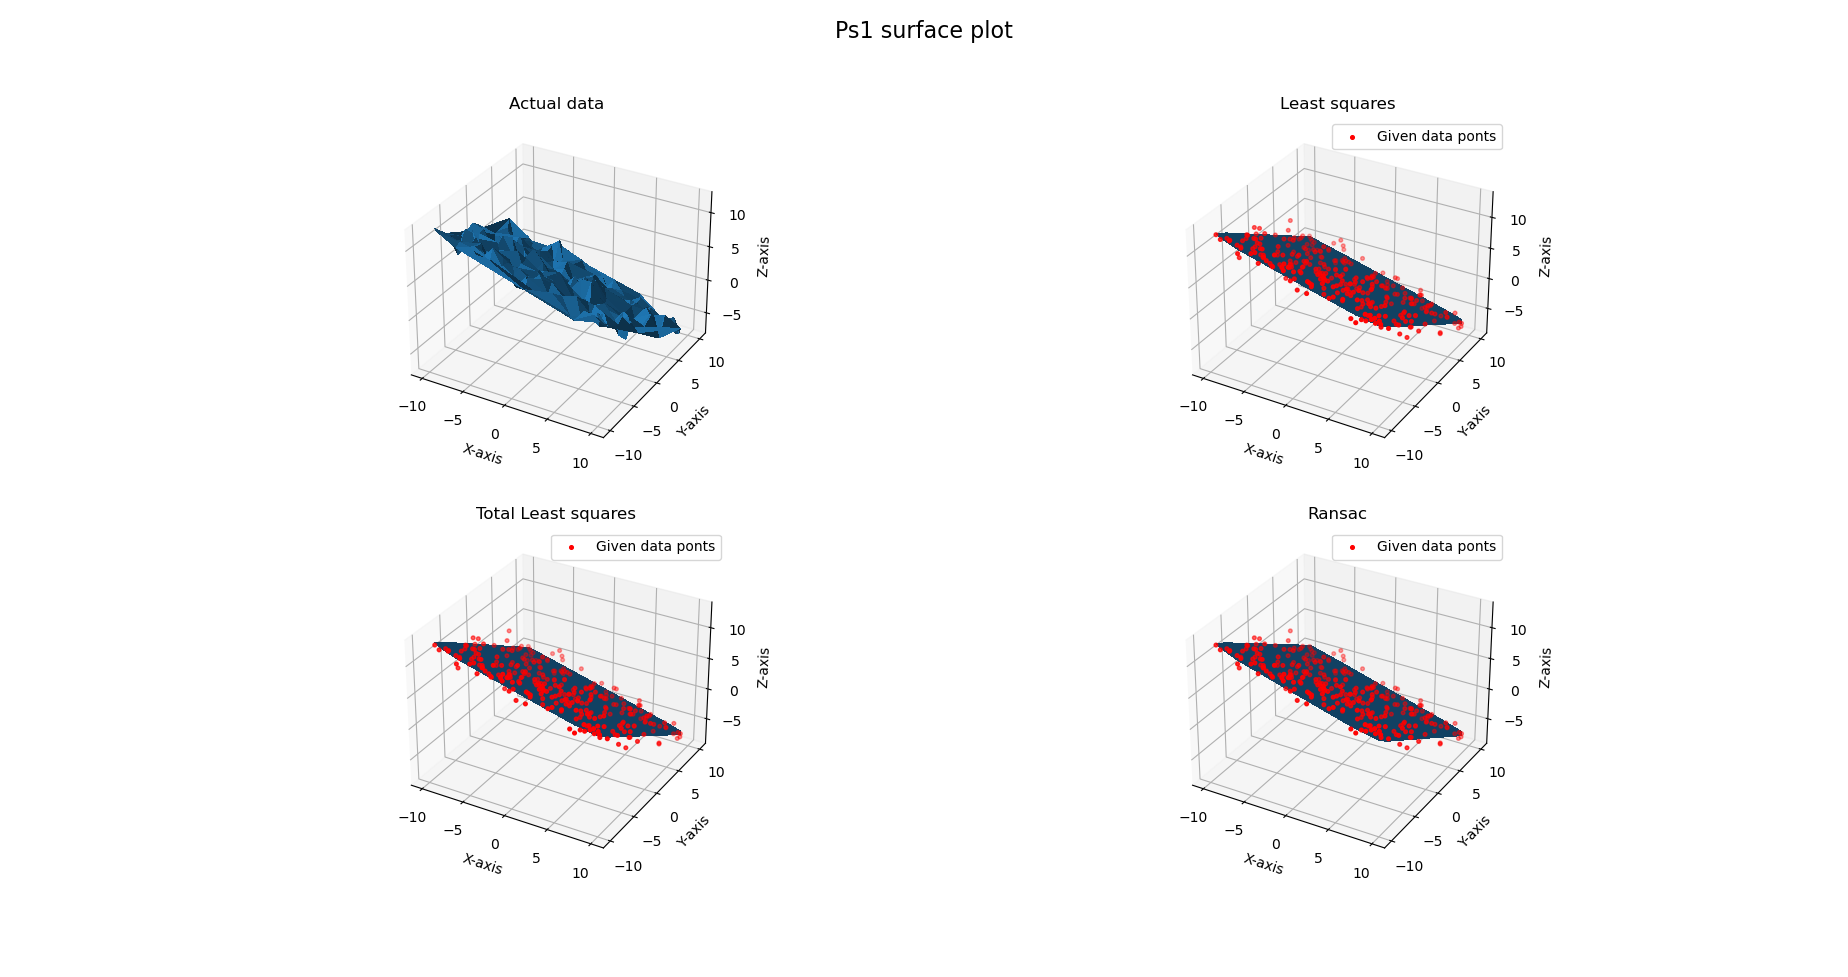
\includegraphics[width= 1.2\textwidth, trim= 8.5cm 0 0 0]{txt/Proj1_2ps1.png}
    \caption{Ps1 surface fit}
    \label{fig:my_label}
\end{figure}

\begin{figure}[!h]
    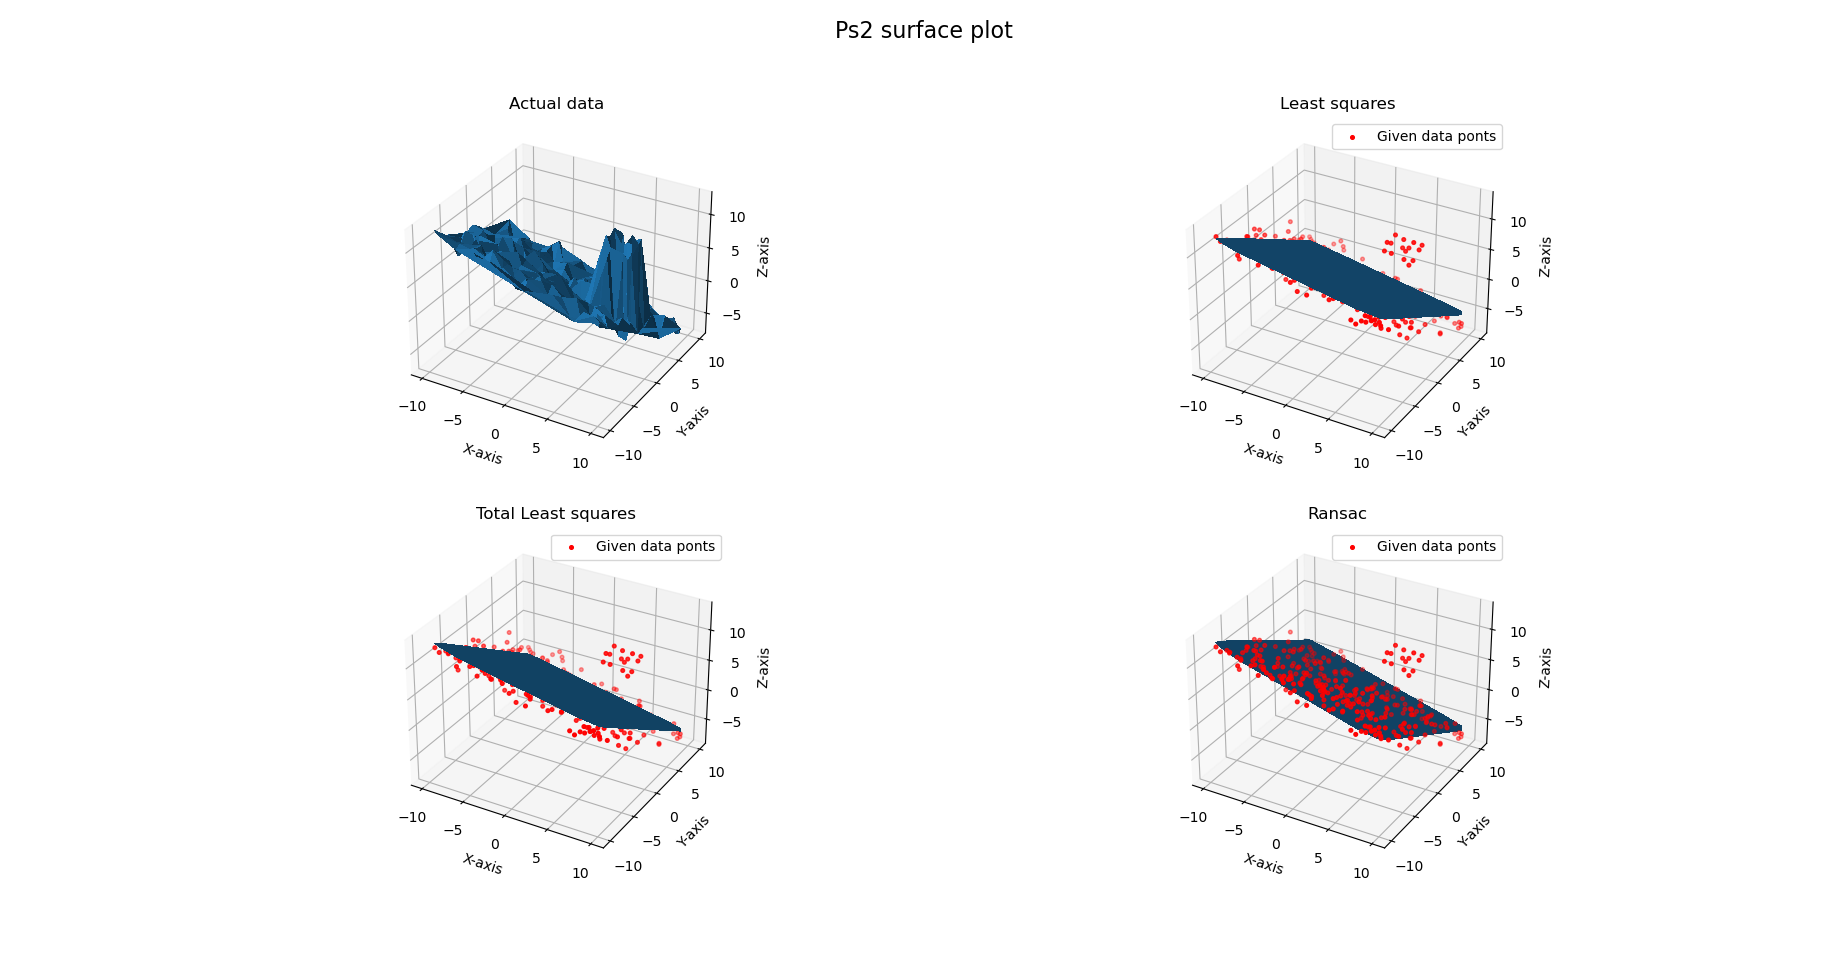
\includegraphics[width= 1.2\textwidth, trim= 8.5cm 0 0 0]{txt/Proj1_2ps2.png}
    \caption{Ps2 surface fit}
    \label{fig:my_label}
\end{figure}

\section{Observations and Interpretation of results}
    When the data is noisy total least squares approach gave a best result than the least squares. The plot of both methods is almost similar and is hard to find differences. And, on the whole, the RANSAC method gave the best model when the data is noisy. By looking at the ps2 data set plots below, we can clearly conclude that the RANSAC method gave the best model. One thing I noticed is that RANSAC generates different sets of a, b, and c values for each run. But the difference in the values of a, b, and c in each run lies in a small range. We can produce, the same values by increasing the number of iterations, but it is not preferred because it slows down the program, If we increase the number of iterations and tune the probability values we can get the desired values of in-liners. For the ps1 dataset, each and every method produced similar kinds of results, but there is a major difference in the second dataset where RANSAC gave the best result. For outlier rejection, RANSAC is the best model.
\pagebreak

\section{Problems Encountered}
\begin{enumerate}
    \item The main problem encountered while ball tracking is getting the upper and lower threshold limits for the mask to filter the red channel. After several iterations and inputs, finally found the correct limit to extract the red channel.
    \item Another problem encountered while ball tracking is in some frames the red channel is not filtered and the values of pixel coordinates are zero, therefore calculating the mean for those values threw an error. The issue got solved after implementing an if condition to leave empty sets.
    \item In the total least squares method, after getting the eigen vector corresponding to the smallest eigen value and while assigning them to the variables a, b, and c it got stored as an array and created a problem while calculating the new z values. A minor change resolved the error, which is converting the 1D array to float.
    \item While performing RANSAC, the no of samples calculation gave an error since the probability values which were given as input made the denominator zero. After changing the probability values, the issue got resolved.
\end{enumerate}


\end{document}

%%%%%%%%%%%%%%%%%%%%%%%%%%%%%%%%%%%%%%%%

% Copyright Remarks:
%--------------------

% Copyright holder: Vebjørn S. Førde, copyright: CC BY 4.0
% Note: The author of this template is also the copyright holder.

% Below is an explanation of the CC BY 4.0. Additional statements/ 
% clarifications made by the author/copyright holder are marked with *.

% YOU ARE FREE TO:
% Share — copy and redistribute the material in any medium or format
% Adapt — remix, transform, and build upon the material
% for any purpose, even commercially.

% UNDER THE FOLLOWING TERMS:
% Attribution* — You must give appropriate credit, provide a link to the license,
% and indicate if changes were made. You may do so in any reasonable manner, but 
% not in any way that suggests the licensor endorses you or your use.

% *Note: 
% Attribution NOT NEEDED for: 
%       - PDF distibution (like sharing your PDF document)
%       - Use of (dummy)text and images provided in the template (obviously)
%       - Distributing parts of the template, and not the template as a whole
% I am not really concerned with being given credit. As long as you do not 
% claim to have made the template yourself in distributing it further, I have
% no complaints.

% No additional restrictions — You may not apply legal terms or technological 
% measures that legally restrict others from doing anything the license permits.

% NOTICES:
% No warranties are given.

% Disclaimer* (added by copyright holder):
% THE SOFTWARE IS PROVIDED "AS IS", WITHOUT WARRANTY OF ANY KIND, EXPRESS OR
% IMPLIED, INCLUDING BUT NOT LIMITED TO THE WARRANTIES OF MERCHANTABILITY,
% FITNESS FOR A PARTICULAR PURPOSE AND NONINFRINGEMENT. IN NO EVENT SHALL THE
% AUTHORS OR COPYRIGHT HOLDERS BE LIABLE FOR ANY CLAIM, DAMAGES OR OTHER
% LIABILITY, WHETHER IN AN ACTION OF CONTRACT, TORT OR OTHERWISE, ARISING FROM,
% OUT OF OR IN CONNECTION WITH THE SOFTWARE OR THE USE OR OTHER DEALINGS IN THE
% SOFTWARE.

% Read more about CC BY 4.0:
% https://creativecommons.org/licenses/by/4.0/